\chapter{Consistency-preserving Visual Question Answering in Medical Imaging}
\label{chapter:cons_mainsub}
% MICCAI 2022 paper about consistency by including annotations about main and sub

Since \gls{vqa} models can be asked multiple questions about the same image, one important aspect of their behavior is what constraints there should be in the answers, given that the questions are related. This is, what level of agreement there should be in the answers so that these do not produce a contradiction. Most of the research in \gls{medvqa} has been focused on improving architectures and working with limited data, while consistency has been overlooked.  

In this work, we tackle the issue of inconsistency in \gls{medvqa} by using a novel loss function term and corresponding training strategy that allows us to consider relations between question-answer pairs in the training process. Following previous approaches from natural images, we examine the case in which the relation between reasoning and perception questions is known. We evaluate our proposed approach on the task of \gls{dme} staging from fundus images. Our experimental results show that our approach enhances not only the consistency of the model but also the overall performance.


\textbf{Author Contribution} This work was co-authored with Pablo Márquez-Neila and Raphael Sznitman. My contributions include the dataset creation, the formulation and implementation of the method, the experimental setup, result analysis and visualization, and the composition of the manuscript. 

\textbf{Publication} This work is published in the Proceedings of the MICCAI 2022 conference~\cite{tascon2022consistency}.

\newpage

% Paper contents
\section{Background and Previous Work}
\label{sec:mainsub_intro}

\gls{vqa} models are neural networks that answer natural language questions about an image by interpreting the question and the image provided~\cite{antol2015vqa,goyal2017making,hudson2019gqa,tan2019lxmert}. Specifying questions using natural language gives \gls{vqa} models great appeal, as the set of possible questions one can ask is enormous and does not need to be identical to the set of questions used to train the models. Due to these advantages, \gls{vqa} models for medical applications have also been proposed~\cite{gong2021cross,ImageCLEFVQA_Med2018,liao2020aiml,liu2019effective,vu2020question,zhan2020medical}, whereby allowing clinicians to probe the model with subtle differentiating questions and contributing to build trust in predictions.

To date, much of the work in \gls{medvqa} has focused on building more effective model architectures~\cite{gong2021cross,liao2020aiml,vu2020question} or overcoming limitations in \gls{medvqa} datasets~\cite{Nguyen19,liao2020aiml,sarrouti2020nlm,zhan2020medical}. Yet a critical component of \gls{vqa} is the notion of {\it consistency} in the answers produced by a model. Here, consistency refers to a model's capacity to produce answers that are not self-contradictory. For instance, the task of staging \gls{dme} from color fundus photograph illustrated in Fig.~\ref{fig:motivation} involves identifying {\it perception} elements in the image (\eg,~``are there hard exudates visible near the macula?'') to infer a disease stage, which can be expressed as a {\it reasoning} question (\eg,~``what is the stage of disease?''). Ultimately, for any \gls{vqa} model to be trustworthy, it should be able to answer these without contradicting itself (\ie, answer that the image is healthy, but also identify hard exudates in the periphery of the eye).
\begin{figure}[t]
\begin{center}
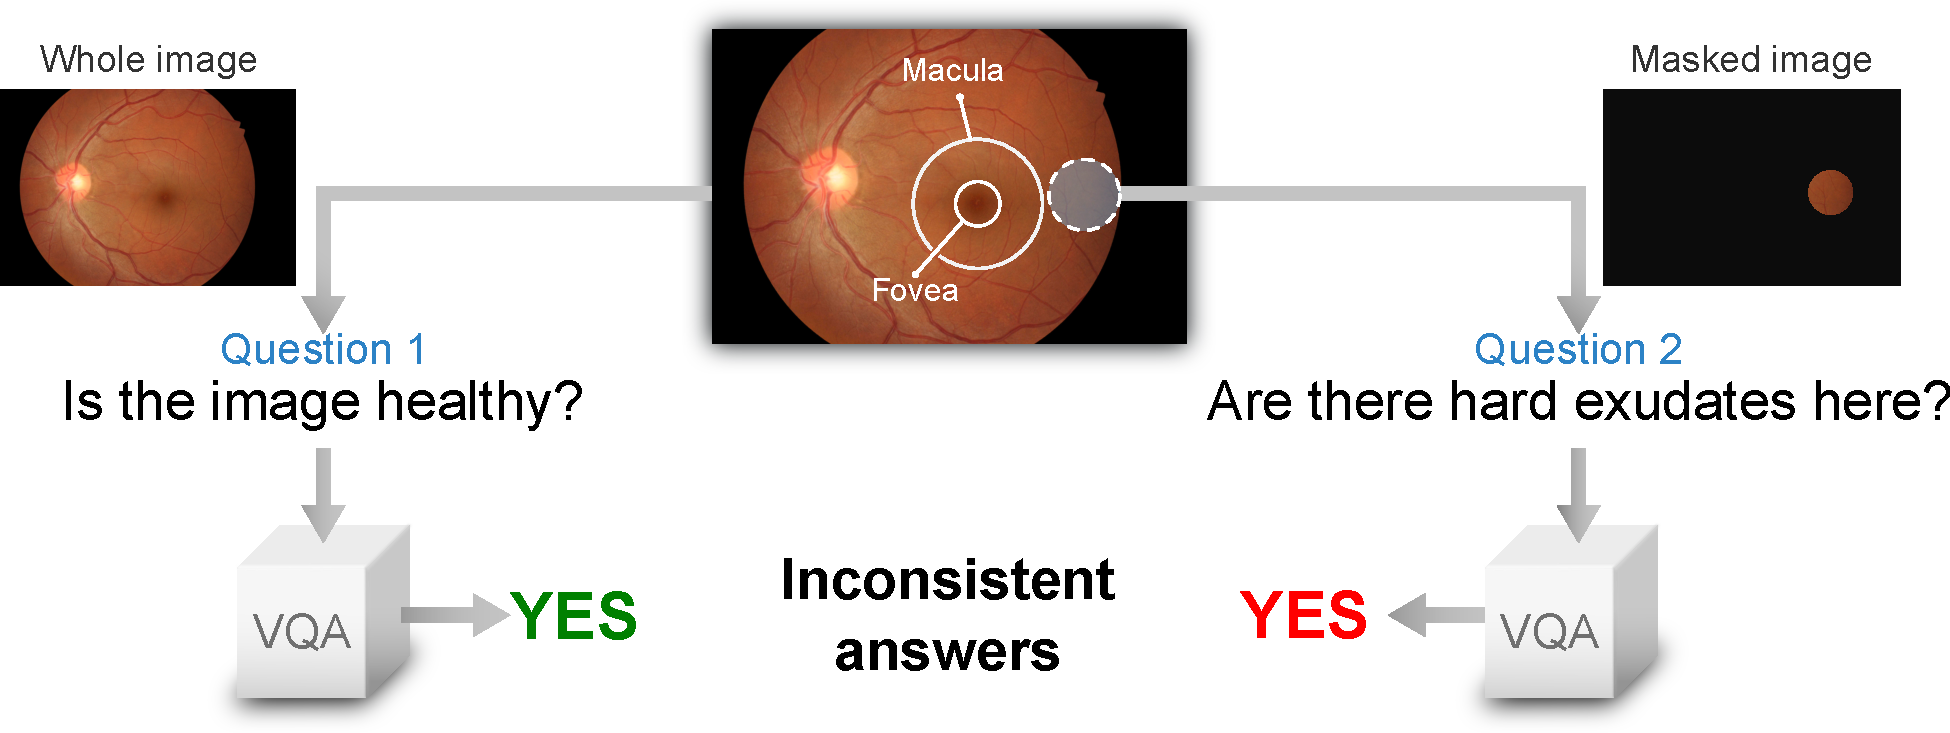
\includegraphics[width=0.75\textwidth]{Figures/Part2_Consist/01_mainsub/motivation_alt.pdf}
\caption{VQA inconsistency in Diabetic Macular Edema staging from fundus photograph. While the VQA model correctly answers ``Is the image healthy?" (left), it incorrectly answers yes to ``Are there hard exudates here?" for a specified retinal region (right).}
\label{fig:motivation}
\end{center}
\end{figure}

\nocite{wang2021image}

Consistency in \gls{vqa} has been been studied in the broader computer vision context~\cite{goel2021iq,gokhale2020vqa,ray2019sunny,ribeiro2019red,shah2019cycle}, where the relation between perception and reasoning questions is unconstrained. That is, the answers to perception questions do not necessarily imply any information with respect to the reasoning question and vice-versa. In these broad cases, some methods have modeled question implications \cite{ray2019sunny,ribeiro2019red} or rephrased questions~\cite{shah2019cycle} by generating tailored question-answer pairs (\eg,~consistent data-augmentation). Alternatively,~\cite{gokhale2020vqa,teney2019incorporating,yuan2021perception} used relations between questions to impose constraints in the \gls{vqa}'s embedding space. To avoid needing to know the relation between questions,~\cite{selvaraju2020squinting} proposed to enforce consistency by making attention maps of reasoning and perception questions similar to one another. 
However, even though these approaches tackle unconstrained question relations, the ensuring of \gls{vqa} models' consistency remains limited and often reduces the overall performance~\cite{selvaraju2020squinting}.  

Instead, we propose a novel approach to enforce \gls{vqa} consistency that is focused on cases where answers to the perception questions have explicit implications on reasoning question answers and vice-versa (\eg, cancerous cells and severity of cancer found in H\&E staining, or presence of hard exudates and \gls{dme} staging). By focusing on this subset of question relations, our aim is to improve both the accuracy of our model and its consistency, without needing external data as in~\cite{ribeiro2019red,Nguyen19,goel2021iq}. To do this, we allow questions to probe arbitrary image regions by masking irrelevant parts of the image and passing the masked image to the \gls{vqa} model (see Fig.~\ref{fig:motivation}). To then enforce consistency, we propose a new loss function that penalizes incorrect perceptual predictions when reasoning ones are correct for a given image. To validate the impact of our approach, we test it in the context of \gls{dme} staging and show that it outperforms state-of-the-art methods for consistency, without compromising overall performance accuracy. 
\section{Method}
\label{sec:mainsub_method}

We present here our approach, which consists of using a simple \gls{vqa} model with a training protocol that encourages consistency among pairs of perception and reasoning questions. Fig.~\ref{fig:method_mainsub} illustrates this \gls{vqa} model and our training approach.

\subsection{VQA Model} Following~\cite{cadene2019rubi}, our \gls{vqa} model,~$f:\mathcal{I}\times\mathcal{Q}\to \mathcal{P}(\mathcal{A})$, takes a tuple containing an image,~$\x$, and a question,~$\q$, to produce a distribution,~$\p=f(\x,\q)$, over a finite set of possible answers~$\mathcal{A}$ (see Fig.~\ref{fig:method_mainsub}(Top)). After encoding the inputs, the \gls{vqa} model combines visual ($v$) and textual ($q$) features through an attention module ($k$)~\cite{xu2015show} that selects the visual features relevant to the question ($v'$). The final classifier receives a combination of the relevant features and the text features through a fusion module to predict the final distribution.

In some cases, questions may be asking about content related to specific regions of the image (\eg, ``are there hard exudates in this region?''). To process these cases, the input image is masked so that the visible area corresponds to the region mentioned in the question while the rest of the image is set to zero.

Training this model requires a dataset~$\mathcal{T}=\{t^{(i)}=(\x^{(i)}, \q^{(i)}, a^{(i)})\}_{i=1}^N\subseteq\mathcal{I}\times\mathcal{Q}\times\mathcal{A}$ of images and questions annotated with their answers. The \gls{vqa}~loss is simply the cross-entropy between the predicted distribution and the real answer,
\begin{equation}
    \label{eq:vqa_loss}
    \ell_{\textrm{VQA}}(\p, a) = H(\p, a) = -\log \p_a.
\end{equation}
While this loss alone is sufficient to reach a reasonable performance, it ignores the potentially useful interactions that may exist among training questions.
\begin{figure}[!h]
\begin{center}
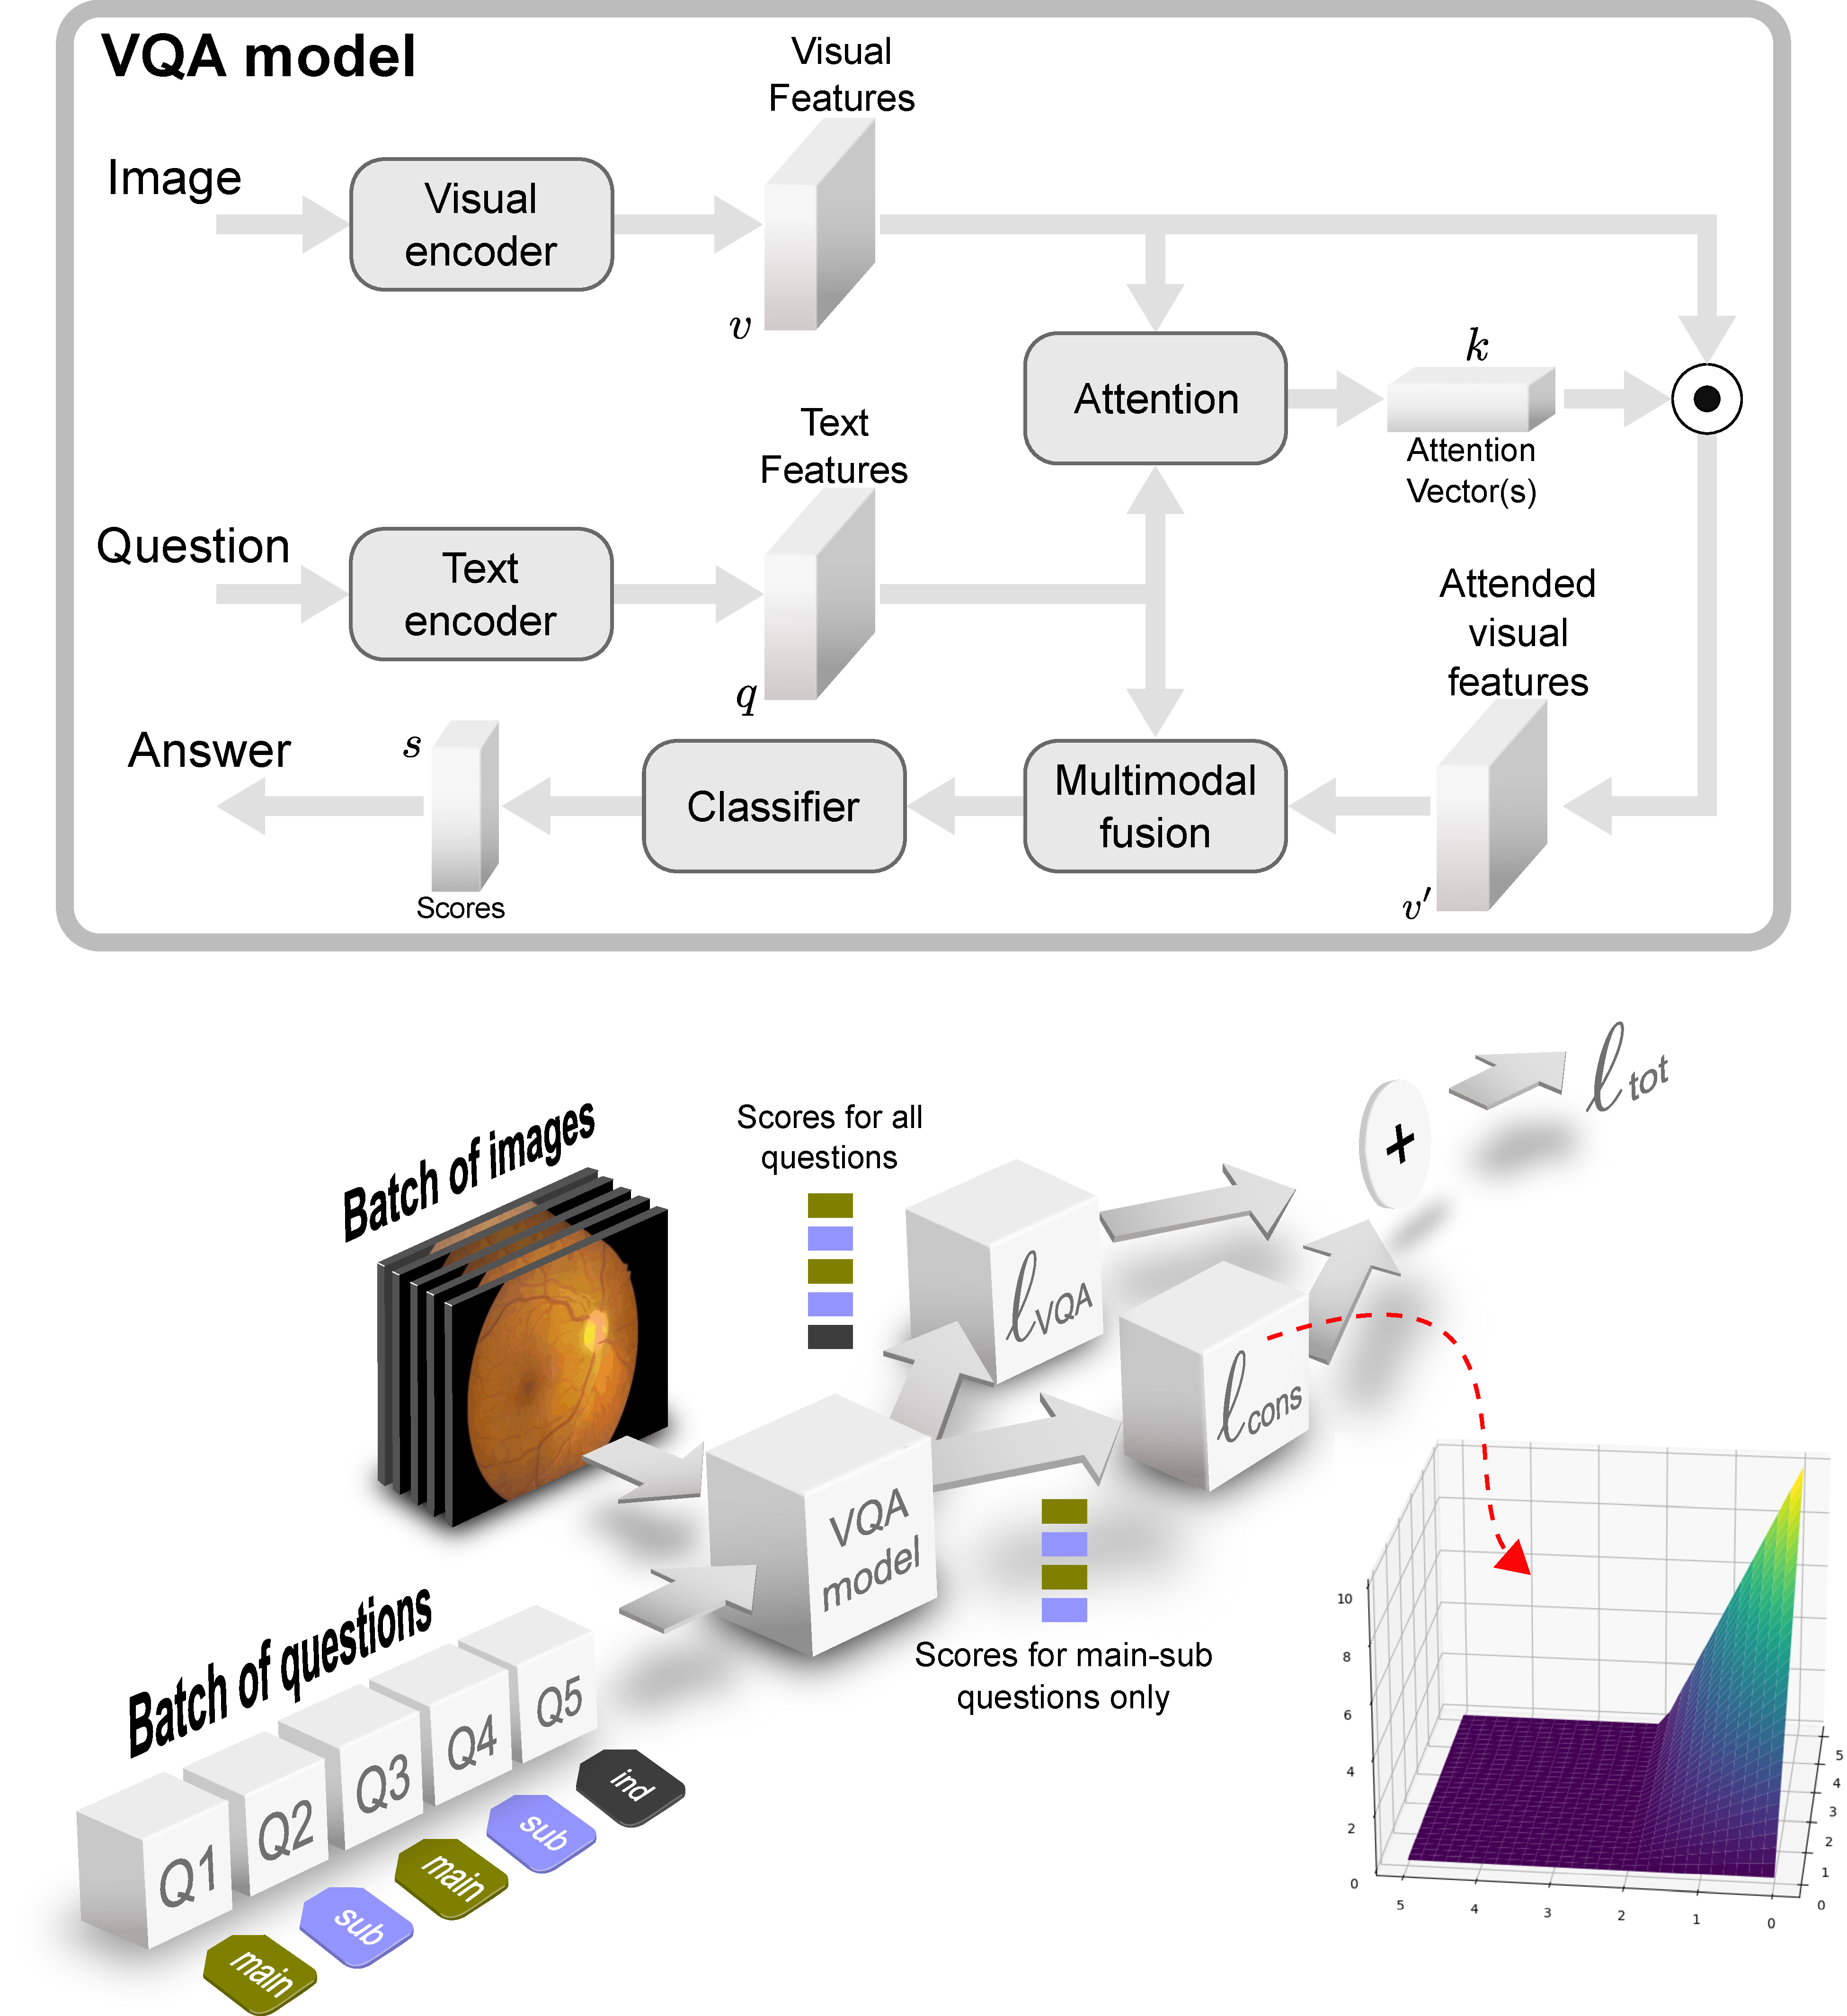
\includegraphics[width=0.75\textwidth]{Figures/Part2_Consist/01_mainsub/method.pdf}
\caption{\textbf{Top:} VQA model architecture. \textbf{Bottom:} Visualization of the training process with the proposed loss. The total loss, $\ell_{\textrm{tot}}$, is based on two terms: the conventional VQA loss,  $\ell_{\textrm{VQA}}$ and our proposed consistency loss term, $\ell_{\textrm{cons}}$. The latter is computed only for pairs of main (reasoning) and sub (perception) questions. Training mini-batches consist of main and sub-questions at the same time, whereby sub-questions can consider specific regions of the image. Unrelated questions (denoted with ``ind") can also be included in training batches but do not contribute to $\ell_{\textrm{cons}}$.}
\label{fig:method_mainsub}
\end{center}
\end{figure}


\subsection{Consistency Loss} We aim to improve the quality of our \gls{vqa} model by exploiting the relationships between reasoning and perception questions at training time. To this end, we augment the training dataset with an additional binary relation~$\prec$ over the set of questions~$\mathcal{Q}$. Two questions are related, $\q^{(i)}\prec \q^{(j)}$, if $\q^{(i)}$ is a perception question associated to the reasoning question~$\q^{(j)}$. From hence on, we refer to perception questions as \emph{sub-questions} and reasoning questions as \emph{main questions}.

Following the terminology in~\cite{selvaraju2020squinting}, an inconsistency occurs when the \gls{vqa} model infers the main question correctly but the sub-question incorrectly. Using the entropy as a measurement of incorrectness, we propose to impose the consistency at training time by penalizing the cases with high $H^{(i)}=H(\p^{(i)}, a^{(i)})$ and low $H^{(j)}=H(\p^{(j)}, a^{(j)})$ when $\q^{(i)}\prec \q^{(j)}$. To do this, we use an adapted hinge loss that disables the penalty when $H^{(j)}$ is larger than a threshold~$\gamma>0$, but otherwise penalizes large values of~$H^{(i)}$,
\begin{equation}
    \label{eq:cons_loss}
    \ell_{\textrm{cons}}(H^{(i)}, H^{(j)}) = H^{(i)}\max\{0, \gamma - H^{(j)}\}.
\end{equation}
\noindent
%$\gamma \in \mathbb{R}^+$. Fig.~\ref{fig:method_mainsub}(Bottom) illustrates $\ell_{\textrm{cons}}$. 

The final cost function then minimizes the expected value of the \gls{vqa} loss~\eqref{eq:vqa_loss} for the elements of the training dataset and the consistency loss~\eqref{eq:cons_loss} for the pairs of training samples with $\prec$-related questions,
\begin{equation}
    \label{eq:cost}
    \mathbb{E}_{t\sim\mathcal{T}}[\ell_\textrm{VQA}(\p, a)] +
    \lambda\mathbb{E}_{(t^{(i)}, t^{(j)})\sim\mathcal{T}^2}[\ell_\textrm{cons}(H^{(i)}, H^{(j)}) \mid \x^{(i)}=\x^{(j)}, \q^{(i)}\prec\q^{(j)}],
\end{equation}
where $\lambda > 0$ controls the relative strength of both losses and $\mathcal{T}^2$ is the Cartesian product of $\mathcal{T}$ with itself, that is, all pairs of training samples.

To train, this cost is iteratively minimized approximating the expectations with mini-batches. The two expectations of Eq.~\eqref{eq:cost} suggest that two mini-batches are necessary at each iteration: one mini-batch sampled from~$\mathcal{T}$ and a second mini-batch of $\prec$-related pairs sampled from $\mathcal{T}^2$. However, in practice a single mini-batch is sufficient as long as we ensure that it contains pairs of $\prec$-related questions. While this biased sampling could in turn bias the estimation of the first expectation, we did not observe a noticeable impact in our experiments. Fig.~\ref{fig:method_mainsub}(Bottom) illustrates this training procedure.
\section{Experiments and Results}

\subsection{DME Staging}
\gls{dme} staging from color fundus images involves grading images on a scale from 0 to 2, with 0 being healthy and 2 being severe (see Fig.~\ref{fig:dme}). Differentiation between the grades relies on the presence of hard exudates present in different locations of the retina. Specifically, a grade of 0 implies that no hard exudates are present at all, a grade of 1 implies that hard exudates are located in the retina periphery (\ie,~outside a circular region centered at the fovea center with radius of one optic disc diameter), and a grade of 2 when hard exudates are in the macular region~\cite{ren2018diabetic}.
\begin{figure}[b!]
\begin{center}
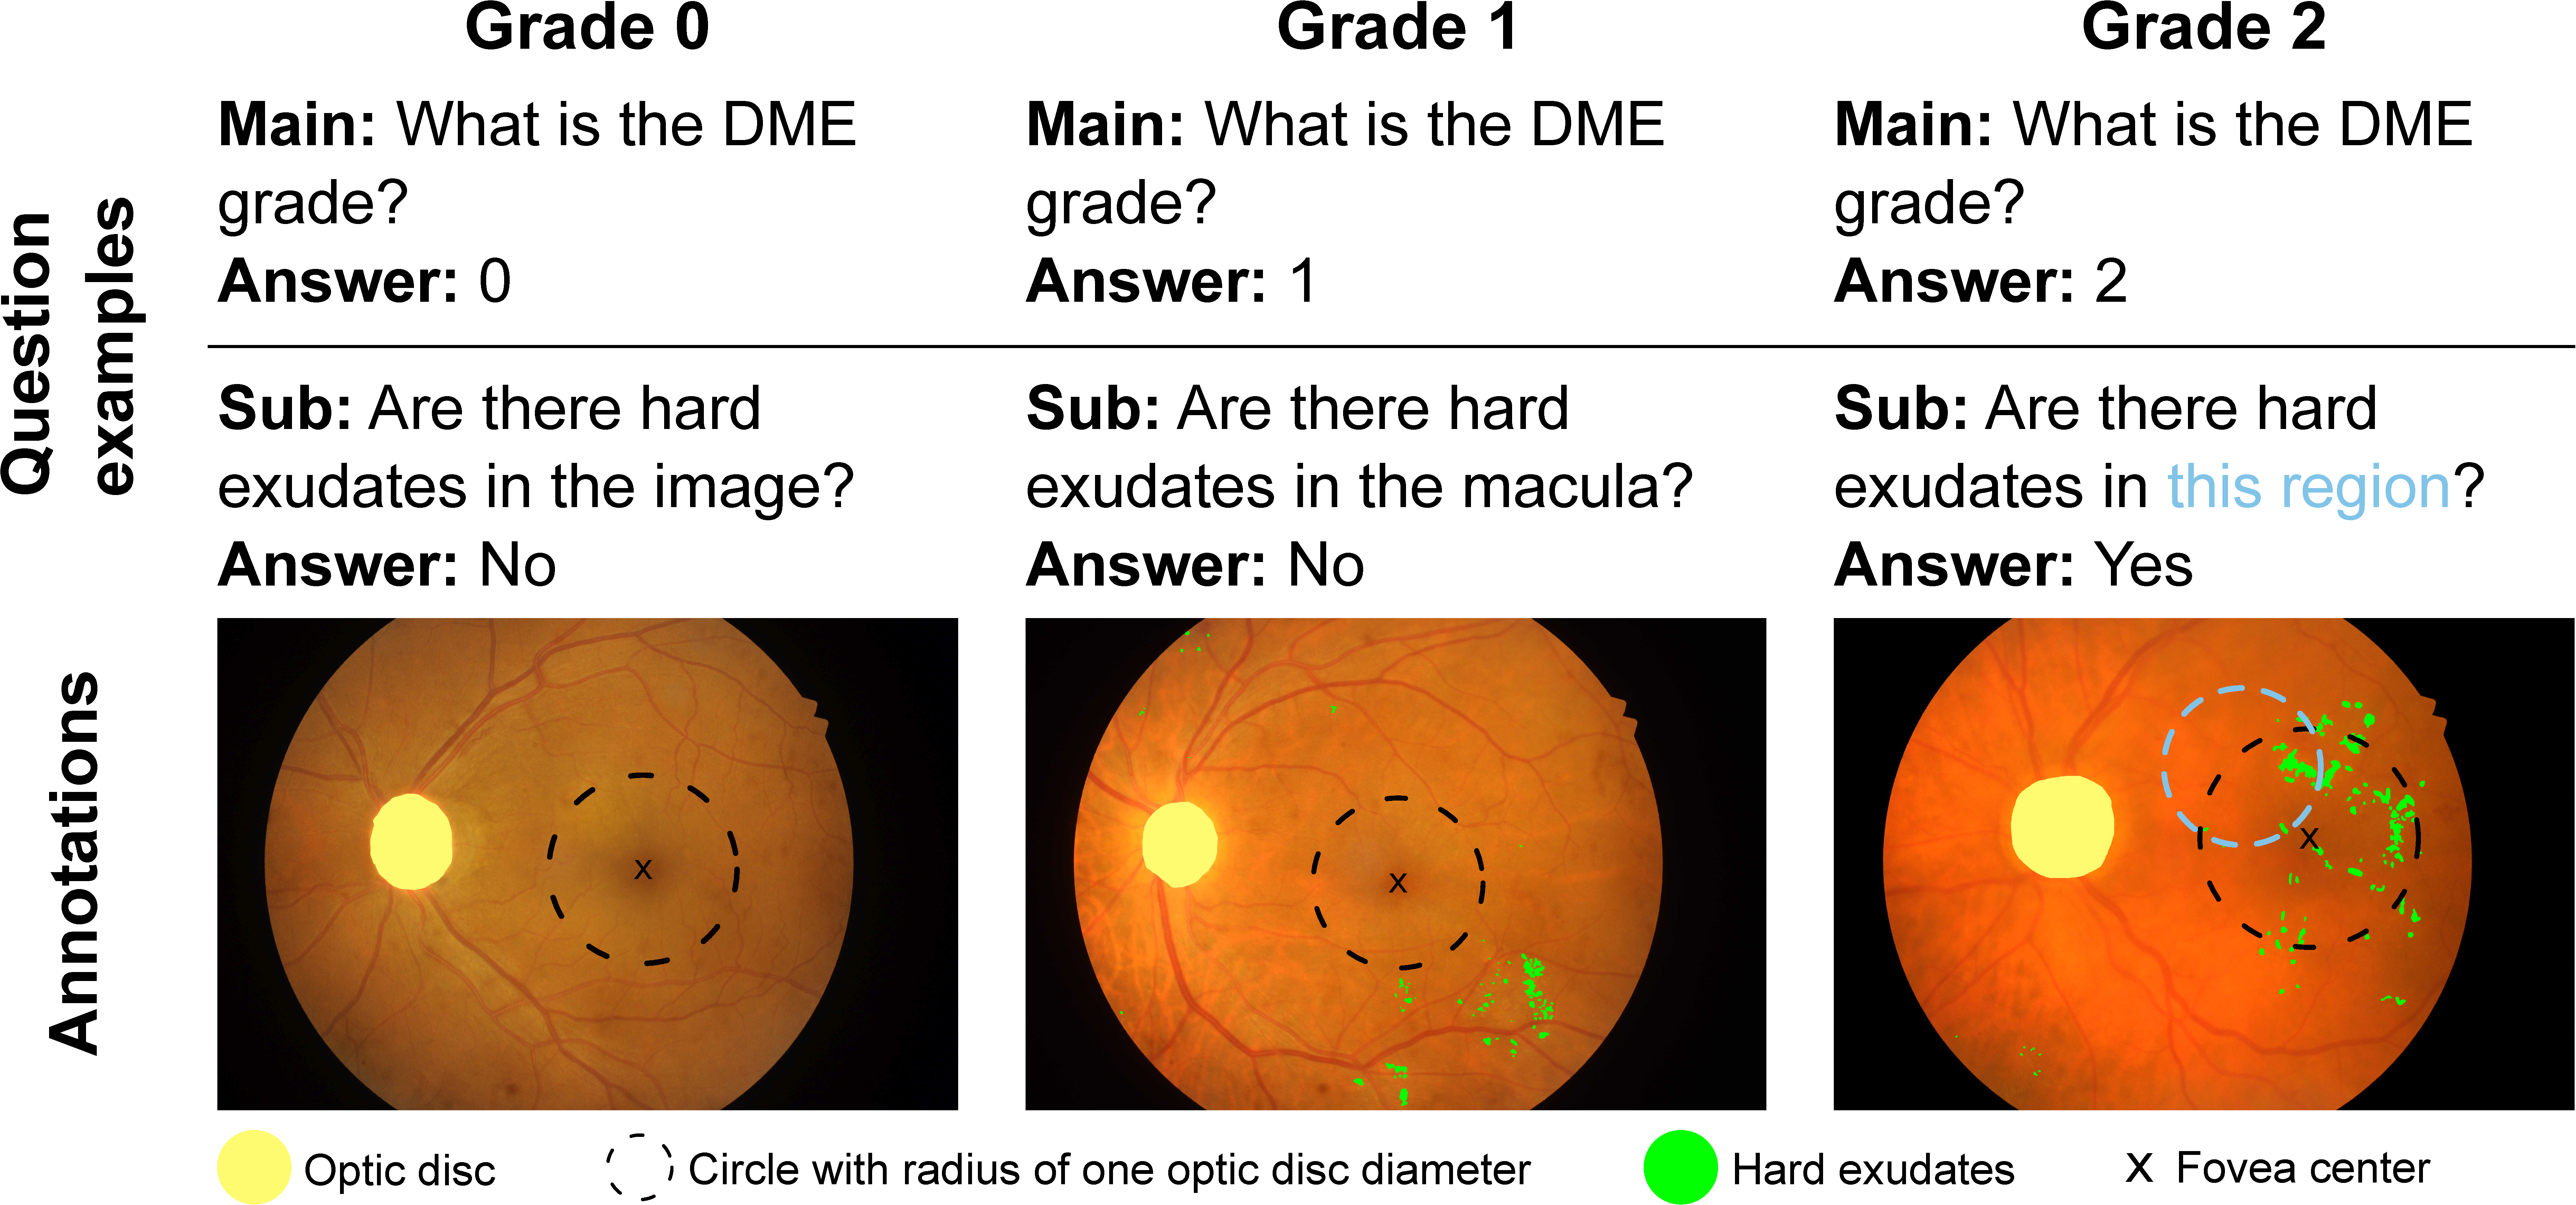
\includegraphics[width=0.9\textwidth]{Figures/Part2_Consist/01_mainsub/dme_2.pdf}
\caption{DME risk grading. Grade 0 is assigned if there are no hard exudates present in the whole image. Grade 1 is assigned if there are hard exudates, but only located outside a circle centered at the fovea with radius of one optic disc diameter. Grade 2 is assigned if there are hard exudates located within the circle. Examples of main and sub-questions are provided for each grade.}
\label{fig:dme}
\end{center}
\end{figure}

\subsection{Dataset}
To validate our method, we make use of two publicly available datasets: the Indian Diabetic Retinopathy Image Dataset (IDRiD)~\cite{idrid} and the e-Ophta dataset~\cite{decenciere2013teleophta}. From the IDRiD dataset, we use images from the segmentation and grading tasks, which consist of 81 and 516 images, respectively. Images from the segmentation task include segmentation masks for hard exudates and images from the grading task only have the \gls{dme} grade. On the other hand, the e-Ophta dataset comprises 47 images with segmentation of hard exudates and 35 images without lesions. Combining both datasets yields a dataset of 128 images with segmentation masks for hard exudates and 128 images without any lesions, plus 423 images for which only the \gls{dme} risk grade is available. 

In this context, we consider main questions to be those asking ``What is the \gls{dme} risk grade?" when considering the entire image. Sub-questions were then defined as questions asking about the presence of the hard exudates. For instance, as shown in Fig.~\ref{fig:dme}{(Right)}, ``Are there hard exudates in this region?" where the region designated contains the macula. In practice, we set three types of sub-questions: ``are there hard exudates in this image?", ``are there hard exudates in the macula?" and ``are there hard exudates in this region?". We refer to these three questions as \textit{whole}, \textit{macula} and \textit{region} questions, respectively. For the region sub-questions, we consider circular regions that can be centered anywhere, or centered on the fovea, depending on availability of fovea center location annotations. As mentioned in Sec.~\ref{sec:mainsub_method}, to answer questions about regions, images are masked so that only the region is visible.

The total number of question-answer pairs in our dataset consists of 9779 for training {(4.4\% main, 21.4\% sub, 74.2\% ind)}, 2380 for validation {(4.5\% main, 19.2\% sub, 76.3\% ind)} and 1311 for testing {(10\% main, 46.1\% sub, 43.9\% ind)}, with images in the train, validation and test sets being mutually exclusive.

\subsection{Experimental Setup}

We compare our approach to a baseline model that does not use the proposed $\ell_{\textrm{cons}}$ loss, equivalent to setting $\lambda=0$. In addition, we compare our method against the attention-matching method, SQuINT~\cite{selvaraju2020squinting}, as it is a state-of-the-art alternative to our approach that can be used with the same \gls{vqa} model architecture.

Our \gls{vqa} model uses an ImageNet-pretrained ResNet101~\cite{he2016deep} with input image of $448\times 448$~pixels and an embedding of 2048~dimensions for the image encoding. For text encoding, a single-layer \gls{lstm}~\cite{hochreiter1997long} network processes the input question with word encoding of length 300 and produces a single question embedding of 1024~dimensions. The multi-glimpse attention mechanism~\cite{xu2015show} uses 2~glimpses and dropout rate~$0.25$, and the multimodal fusion stage uses standard concatenation. The final classifier is a multi-layer perceptron with hidden layer of 1024 dimensions and dropout rate of 0.25. Hyperparameters~$\lambda$ and~$\gamma$ were empirically adjusted to 0.5 and~1.0, respectively. 

All experiments were implemented using PyTorch~1.10.1 and run on a Linux machine with an NVIDIA RTX 3090 graphic card using 16~GB of memory and 4~CPU cores. All methods use the weighted cross-entropy as the base \gls{vqa} loss function. Batch size was set to~64, and we used Adam for optimization with a learning rate of $10^{-4}$. Maximum epoch number was 100 and we use early stopping policy to prevent overfitting, with patience of 20~epochs \footnote{Our code and data are available at \url{https://github.com/sergiotasconmorales/consistency_vqa}}.

We report accuracy and consistency~\cite{selvaraju2020squinting} performances, using two different definitions of consistency for comparison. Consistency, C1, is the percentage of sub-questions that are answered correctly when the main question was answered correctly. Consistency, C2, is the percentage of main questions that are answered correctly when all corresponding sub-questions were answered correctly.

\subsection{Results}
Table \ref{tab:results} shows the results.
% for the best values of the hyperparameters $\lambda$ and $\gamma$. \RS{I don't understand this. Do we have other values of $\lambda$ and $\gamma$. Do we have that as well for Squint}.
We compare these results to the case in which the value of $\lambda$ is~0, which corresponds to the baseline in which no additional loss term is used. For each case, we present the overall accuracy and the accuracy for each type of question, as well as the consistency values. Fig.~\ref{fig:examples} illustrates the performance of each method with representative qualitative examples.


\begin{table}[!t]
\begin{center}
\resizebox{\textwidth}{!}{
\begin{tabular}{llllllll}
\toprule
\multicolumn{1}{l}{\multirow{2}{*}{Case}}    &  \multicolumn{5}{c}{Accuracy} & \multicolumn{2}{c}{Consistency} \\ \cline{2-8} \multicolumn{1}{c}{}  
                   & \multicolumn{1}{l}{overall}      & \multicolumn{1}{l}{grade}        & \multicolumn{1}{l}{whole}        & \multicolumn{1}{l}{macula}       & \multicolumn{1}{l}{region}       & \multicolumn{1}{c}{C1}            & \multicolumn{1}{c}{C2}          

\\ \hline
\multicolumn{1}{l}{Baseline (no att.)}                                 & \multicolumn{1}{l}{77.54 } & \multicolumn{1}{l}{73.59} & \multicolumn{1}{l}{81.37 } & \multicolumn{1}{l}{83.37}& \multicolumn{1}{l}{76.66 } & \multicolumn{1}{l}{81.70 }  & \multicolumn{1}{l}{91.86 } 

\\ 
\multicolumn{1}{l}{Baseline (att.)}                            & \multicolumn{1}{l}{81.46 } & \multicolumn{1}{l}{80.23} & \multicolumn{1}{l}{83.13 } & \multicolumn{1}{l}{\textbf{87.18} }& \multicolumn{1}{l}{80.58 } & \multicolumn{1}{l}{89.21 }  & \multicolumn{1}{l}{96.92 } 

\\ 
\multicolumn{1}{l}{Baseline (att.) + SQuINT~\cite{selvaraju2020squinting}  }                                  & \multicolumn{1}{l}{80.58} & \multicolumn{1}{l}{77.48} & \multicolumn{1}{l}{82.82} & \multicolumn{1}{l}{85.34}& \multicolumn{1}{l}{80.02} & \multicolumn{1}{l}{88.17}  & \multicolumn{1}{l}{94.62} 

\\ 
\multicolumn{1}{l}{Baseline (att.) + Ours ($\lambda=0.5,\gamma=1$)}             & \multicolumn{1}{l}{\textbf{83.49} } & \multicolumn{1}{l}{\textbf{80.69} } & \multicolumn{1}{l}{\textbf{84.96} } & \multicolumn{1}{l}{\textbf{87.18} } & \multicolumn{1}{l}{\textbf{83.16}} & \multicolumn{1}{l}{\textbf{94.20} } & \multicolumn{1}{l}{\textbf{98.12} } 

\\ \bottomrule                  
\end{tabular}
}
\end{center}
\caption{Average test accuracy and consistency values for the different models. Results shown are averaged over 10 models trained with different seeds. Accuracy values are presented for all questions (overall), for main questions (grade) and for sub-questions (whole, macula and region). Both measures of consistency are shown as well.}
\label{tab:results}
\end{table}
\begin{figure}[!t]
\begin{center}
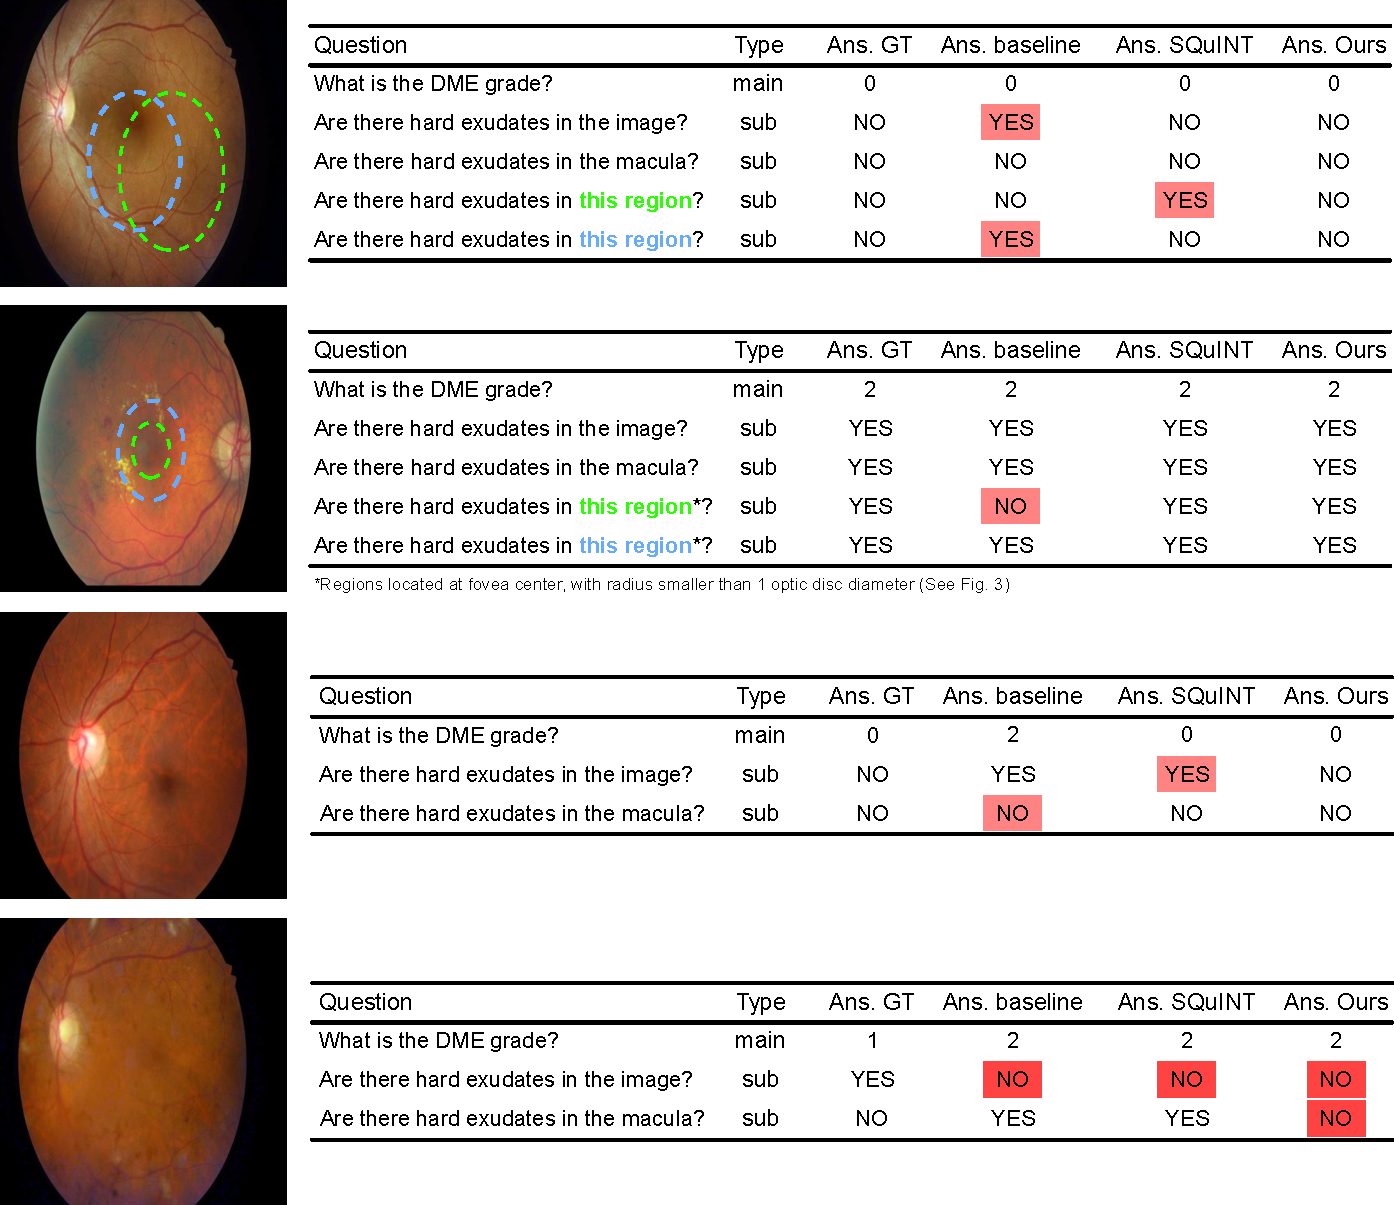
\includegraphics[width=0.99\textwidth]{Figures/Part2_Consist/01_mainsub/examples_expl_marked_add.pdf}
\caption{Qualitative examples from the test set. Inconsistent sub-answers are highlighted in red. Additional examples are shown in Appendix~\ref{appendix:consistency_mainsub}.  
}
\label{fig:examples}
\end{center}
\end{figure}


\begin{table}[!t]
\begin{center}
\begingroup
\setlength{\tabcolsep}{10pt} % Default value: 6pt
\renewcommand{\arraystretch}{1.5} % Default value: 1
\begin{tabular}{lllllllll}
\toprule
 \multicolumn{1}{c}{\multirow{2}{*}{$\lambda$}} & \multicolumn{1}{c}{\multirow{2}{*}{$\gamma$}} & \multicolumn{5}{c}{Accuracy}   & \multicolumn{2}{c}{Consistency}  \\ \cline{3-9} 
\multicolumn{1}{c}{}                         & \multicolumn{1}{c}{}      &  \multicolumn{1}{c}{overall}                       & \multicolumn{1}{c}{grade}      & \multicolumn{1}{c}{whole}        & \multicolumn{1}{c}{macula}        & \multicolumn{1}{c}{region}     & \multicolumn{1}{c}{C1}            & \multicolumn{1}{c}{C2}          
\\ \hline

\multicolumn{1}{l}{0}                     & \multicolumn{1}{l}{-}                    & \multicolumn{1}{l}{81.46} & \multicolumn{1}{l}{80.23} & \multicolumn{1}{l}{83.13} & \multicolumn{1}{l}{87.18} & \multicolumn{1}{l}{80.58} & \multicolumn{1}{l}{89.21} & \multicolumn{1}{l}{96.92} 

\\ \hline 

\multicolumn{1}{l}{0.2}                     & \multicolumn{1}{l}{0.5}                    & \multicolumn{1}{l}{82.01} & \multicolumn{1}{l}{80.38} & \multicolumn{1}{l}{83.59} & \multicolumn{1}{l}{86.56} & \multicolumn{1}{l}{81.36} & \multicolumn{1}{l}{90.93} & \multicolumn{1}{l}{97.38} 

\\ 
\multicolumn{1}{l}{0.2}                     & \multicolumn{1}{l}{1}                    & \multicolumn{1}{l}{82.65} & \multicolumn{1}{l}{ 79.77} & \multicolumn{1}{l}{ 83.97} & \multicolumn{1}{l}{ 86.64} & \multicolumn{1}{l}{82.30} & \multicolumn{1}{l}{ 93.22} & \multicolumn{1}{l}{97.51 } 

\\ 

\multicolumn{1}{l}{0.2}                     & \multicolumn{1}{l}{1.5}                    & \multicolumn{1}{l}{83.05} & \multicolumn{1}{l}{81.22} & \multicolumn{1}{l}{ 84.27} & \multicolumn{1}{l}{ 87.33} & \multicolumn{1}{l}{82.53} & \multicolumn{1}{l}{ 93.23} & \multicolumn{1}{l}{ 97.56} 


\\ \hline 
\multicolumn{1}{l}{0.3}                     & \multicolumn{1}{l}{0.5}                   & \multicolumn{1}{l}{82.34} & \multicolumn{1}{l}{ 79.92} & \multicolumn{1}{l}{ 83.59} & \multicolumn{1}{l}{ 87.71} & \multicolumn{1}{l}{81.74} & \multicolumn{1}{l}{ 92.32} & \multicolumn{1}{l}{ 97.31} 

\\ 

\multicolumn{1}{l}{0.3}                     & \multicolumn{1}{l}{1}                 & \multicolumn{1}{l}{83.27} & \multicolumn{1}{l}{ 80.53} & \multicolumn{1}{l}{ 84.58} & \multicolumn{1}{l}{ 87.25} & \multicolumn{1}{l}{82.91} & \multicolumn{1}{l}{ 94.01} & \multicolumn{1}{l}{ 98.10} 

\\ 

\multicolumn{1}{l}{0.3}                     & \multicolumn{1}{l}{1.5}                   & \multicolumn{1}{l}{83.28} & \multicolumn{1}{l}{80.84 } & \multicolumn{1}{l}{ 84.43} & \multicolumn{1}{l}{ 87.48} & \multicolumn{1}{l}{82.86} & \multicolumn{1}{l}{ 93.28} & \multicolumn{1}{l}{ 98.29} 


\\ \hline 

\multicolumn{1}{l}{0.4}                     & \multicolumn{1}{l}{0.5}                   & \multicolumn{1}{l}{82.87} & \multicolumn{1}{l}{80.69} & \multicolumn{1}{l}{ 84.89} & \multicolumn{1}{l}{ 87.02} & \multicolumn{1}{l}{82.30} & \multicolumn{1}{l}{ 92.66} & \multicolumn{1}{l}{ 96.66} 

\\ 
\multicolumn{1}{l}{0.4}                     & \multicolumn{1}{l}{1}                 & \multicolumn{1}{l}{82.97} & \multicolumn{1}{l}{ 80.15} & \multicolumn{1}{l}{ 83.97} & \multicolumn{1}{l}{ 86.72} & \multicolumn{1}{l}{82.69} & \multicolumn{1}{l}{ 93.91} & \multicolumn{1}{l}{98.23} 

\\ 
\multicolumn{1}{l}{0.4}                     & \multicolumn{1}{l}{1.5}                  & \multicolumn{1}{l}{83.33} & \multicolumn{1}{l}{ 80.08} & \multicolumn{1}{l}{ 84.20} & \multicolumn{1}{l}{ 86.87} & \multicolumn{1}{l}{83.17} & \multicolumn{1}{l}{ 93.96} & \multicolumn{1}{l}{ 97.77} 

\\ \hline 
\multicolumn{1}{l}{0.5}                     & \multicolumn{1}{l}{0.5}                & \multicolumn{1}{l}{82.54} & \multicolumn{1}{l}{81.07 } & \multicolumn{1}{l}{ 83.66} & \multicolumn{1}{l}{ 88.02} & \multicolumn{1}{l}{81.81} & \multicolumn{1}{l}{ 91.87} & \multicolumn{1}{l}{ 97.73} 

\\ 
\multicolumn{1}{l}{0.5}                     & \multicolumn{1}{l}{1}                    & \multicolumn{1}{l}{83.49} & \multicolumn{1}{l}{80.69 } & \multicolumn{1}{l}{84.96 } & \multicolumn{1}{l}{87.18} & \multicolumn{1}{l}{83.16} & \multicolumn{1}{l}{94.20} & \multicolumn{1}{l}{98.12 } 

\\ 
\multicolumn{1}{l}{0.5}                     & \multicolumn{1}{l}{1.5}             & \multicolumn{1}{l}{83.25} & \multicolumn{1}{l}{ 79.92} & \multicolumn{1}{l}{ 84.58} & \multicolumn{1}{l}{ 86.95} & \multicolumn{1}{l}{83.01} & \multicolumn{1}{l}{ 94.20} & \multicolumn{1}{l}{ 98.12} 

\\ \bottomrule                  
\end{tabular}
\endgroup
\end{center}
\caption{Average test accuracy and consistency values for different values of the parameters $\lambda$ and $\gamma$. The first row ($\lambda\, =\, 0$) corresponds to no consistency enhancement method.}
\label{tab:results_params}
\end{table}
In general, we observe that our proposed approach yields increases in accuracy and consistency when compared to both the baseline and SQuINT. Importantly, this increase in consistency is not at the expense of overall accuracy. Specifically, this indicates that our loss term causes the model to be correct about sub-questions when it is correct about main questions. The observed increase in accuracy also indicates that our approach is not synthetically increasing consistency by reducing the number of correct answers on main questions~\cite{selvaraju2020squinting}. We note that SQuINT results in a reduction in accuracy and consistency, which can be partially explained by the presence of region questions that are not associated to any main question. These questions, which exceed the number of main questions, may affect the constraint in the learned attention maps.

Table~\ref{tab:results_params} shows the effect of $\lambda$ and $\gamma$ on the performance metrics. As expected, we notice that when $\lambda$ increases, the consistency of our approach increases as well and will occasionally deteriorate overall accuracy. The impact of $\gamma$ however is less evident, as no clear trend is visible. This would imply that the exact parameter value used is moderately critical to performances. 
\section{Conclusion}

In this work, we presented a novel method for improving consistency in \gls{vqa} models in cases where answers to sub-questions imply those of main questions and vice-versa. By using a tailored training procedure and loss function that measures the level of inconsistency, we show on the application of \gls{dme} staging, that our approach provides important improvements in both \gls{vqa} accuracy and consistency. In addition, we show that our method's hyperparameters are relatively insensitive to model performance. In the future, we plan to investigate how this approach can be extended to the broader case of unconstrained question relations.